\documentclass{beamer}
\usepackage{tcolorbox}
\usepackage{forloop}
\usepackage{textpos}


%\beamerdefaultoverlayspecification{<+->}
\newcommand{\data}{\mathcal{D}}

\DeclareMathOperator*{\argmin}{arg\,min}

\newcommand\Item[1][]{%
	\ifx\relax#1\relax  \item \else \item[#1] \fi
	\abovedisplayskip=0pt\abovedisplayshortskip=0pt~\vspace*{-\baselineskip}}

\newcommand<>{\fullsizegraphic}[1]{
	\begin{textblock*}{0cm}(-1cm,-3.78cm)
		\includegraphics[height=\paperheight]{#1}
	\end{textblock*}
}

\usetheme{metropolis}           % Use metropolis theme


\title{Bayesian Optimization}
\date{\today}
\author{Nipun Batra}
\institute{IIT Gandhinagar}
\begin{document}
  \maketitle
  
%\newcounter{iter}
%\forloop{iter}{1}{\value{iter} < 5}%
%{%
%	\begin{frame}{Bayes Rule - \theiter}
%		\begin{center}
%			\includegraphics[height=\textheight -100pt ,keepaspectratio]{bo-images/pngs/ACQ1/1/\theiter}
%		\end{center}
%	\end{frame}
%}

\section{Primer}
\newcounter{iter}
\forloop{iter}{1}{\value{iter} < 14}%
{%
	\begin{frame}{BO Primer Slide \theiter}
		\begin{center}
			\fullsizegraphic{bo-images/nslides/Slide\theiter}
		\end{center}
	\end{frame}
}

\section{Mining Gold!}
\begin{frame}{Problem Setting}
	We will first start with an example, which is a manifestation of the optimization problems we encounter in the wild.
	
	Our goal is to mine for gold in a new, unknown land. For now, let us make a simplifying assumption, the gold content lies in a one-dimensional space, i.e., we are talking gold distribution only about a line. Let the function be denoted by $f(x)$ where $x$ signifies the location.
	
	We want to find the location with the maximum gold content is situated though one caveat is that the cost of each drilling is too huge.
\end{frame}

\begin{frame}{Problem Specifications}
    As stated above, we would like to find the location of the maximum gold concentration.

	We want to \textbf{minimize the number of drilling required} while still being able to \textbf{find the location of the maximum gold quickly}.
	
	Looking below, we see that the gold distribution is the maximum around $x=5$.
	\begin{center}
		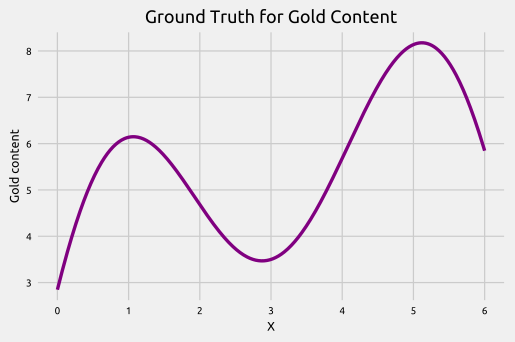
\includegraphics[height=.5\textheight]{bo-images/gifs/GT}
	\end{center}
\end{frame}

\begin{frame}{Surrogate Model}
	\urldef\matern\url{https://scikit-learn.org/stable/modules/generated/sklearn.gaussian_process.kernels.Matern.html}
	
	To model the unknown function we would use Gaussian Process Regressor. This is called the surrogate model.
	
	\begin{center}
		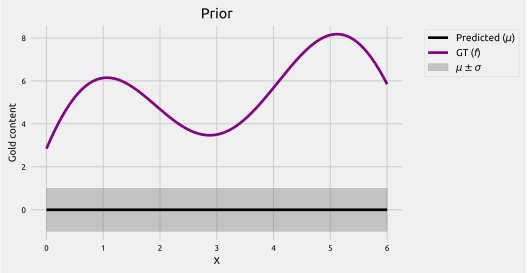
\includegraphics[height=.46\textheight]{bo-images/gifs/prior}
	\end{center}
	
	Initially the GP would not have any information, which can be seen by looking at the prior above. We assume that the gold distribution $f$ is smooth, via a Matern kernel \footnote{\matern}.
\end{frame}

\begin{frame}{Adding Training Data}
	\begin{center}
		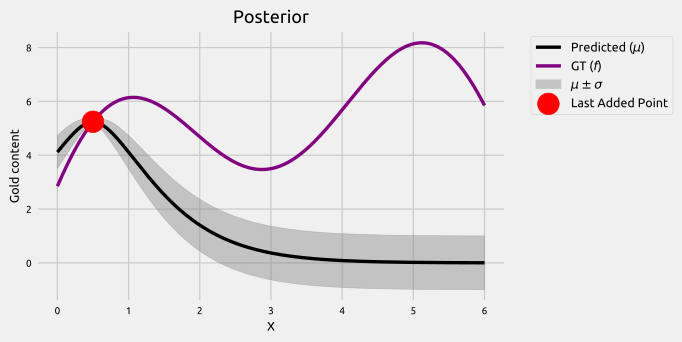
\includegraphics[height=.46\textheight]{bo-images/gifs/posterior}
	\end{center}
	
	We see how adding training point (drilling at a location and actually getting the gold concentration) changed the posterior of our surrogate model.
	
	We see that as more points are sampled, our surrogate is able to model more accurately.
\end{frame}

\section{Formalizing Bayesian Optimization}
\begin{frame}{Idea}
	Our main aim in the example discussed is to find the point where we can get the maximum gold content.
	
	Given this, it might be a good idea to use the information from the surrogate model. It might be likely where the surrogate predicts higher functional value; the functional value is actually higher.    In Essence, one might want to \textbf{exploit}.
	
	But, the surrogate is not a perfect model of $f$. Therefore, one would like to improve the surrogate model too. This is done by getting the functional values at points the surrogate is most uncertain about. This is \textbf{exploration}.
\end{frame} 


% [width=\linewidth]

%\begin{frame}{Bayes Rule - 2}
%\begin{itemize}
%	
%\item Test will produce 99\% true positive results for drug users and 99\% true negative results for non-drug users $\implies$
%\begin{itemize}
%	\item $P(Test=+|User=Drug) = 0.99$, or, $P(+|User) = 0.99$
%	\item and $P(-|\overline{User}) =0.99$ 
%\end{itemize}  
%		\item 0.5\% of people are users of the drug $\implies P(User) = 0.005$
%		\item Question: What is the probability that a randomly selected individual with a positive test is a drug user? $\implies P(User|+) = ?$
%		\item 
%				$P(User|+) = \frac{P(+|User)P(User)}{P(+)} = $
%		\item $\frac{P(\text{+}\mid\text{User}) P(\text{User})}{P(\text{+}\mid\text{User}) P(\text{User}) + P(\text{+}\mid\overline{User}) P(\overline{User})} = \frac{0.99\times 0.005}{0.99\times 0.005 + 0.01\times0.995} \approx .332$ 
%	
%\end{itemize}
%\end{frame}
%
%\begin{frame}{Another example on Bayes rule}
%\end{frame}
%
%
%\begin{frame}{Bayes Rule for Machine Learning}
%\begin{itemize}
%
%
%    \item $P(A|B)P(B) = P(B|A)P(A)$
%    \item Let us consider for a machine learning problem:
%    \begin{itemize}
%    	\item A = Parameters ($\theta$)
%    	\item B = Data ($\mathcal{D}$)
%    \end{itemize}
%\item We can rewrite the Bayes rule as:
%\begin{itemize}
%	\item $P(\theta|\mathcal{D}) = \frac{P(\mathcal{D}|\theta)P(\theta)}{P(\mathcal{D})}$
%	\item Posterior: 
%	\item Prior:
%	\item Likelihood
%	\item 
%\end{itemize}
%\end{itemize}
%\end{frame}
%
%\begin{frame}{Likelihood}
%\begin{itemize}
%	\item Likelihood is a function of $\theta$
%	\item Given a coin flip and 5 H and 1 T, what is more likely: P(H) = 0.5 or P(H) = 1
%\end{itemize}
%\end{frame}
%
%\begin{frame}{Bayesian Learning is well suited for online settings}
%content...
%\end{frame}
%
%\begin{frame}{Coin flipping}
%\begin{itemize}
%	\item Assume we do a coin flip multiple times and we get the following observation: \{H, H, H, H, H, H, T, T, T, T\}: 6 Heads and 4 Tails
%	\item  What is $P(Head)$?
%	\item Is your answer: 6/10. Why?
%\end{itemize}
%
%\end{frame}
%
%\begin{frame}{Coin flipping: Maximum Likelihood Estimate (MLE)}
%\begin{itemize}
%	\item We have $\mathcal{D} = \{\data_1, \data_2, ...\data_{N}\}$ for $N$ observations where each $\mathcal{D}_i \in \{H, T\}$
%	\item Assume we have $n_H$ heads and $n_T$ tails, $n_H + n_T = N$
%	\item Let us have $P(H) = \theta, P(T) = 1-\theta$
%	\item We have Likelihood, $L(\theta) = P(\mathcal{D}|\theta) = P(\data_1, \data_2, ..., \data_N|\theta)$
%	\item Since observations are i.i.d., $L(\theta) = P(\data_1|\theta).P(\data_2|\theta) ... P(\data_N|\theta)$
%\end{itemize}
%
%\end{frame}
%
%
%\begin{frame}{Coin flipping: Maximum Likelihood Estimate (MLE)}
%\begin{itemize}
%	\item  
%\begin{align*}  
%P(\data_i|\theta) =  \left
%\{\begin{array}{lr} \theta, & \text{for~} \data_i =H \\
%1-\theta, & \text{for~} \data_i = T
%\end{array}\right.\
%\end{align*}  
%\item Thus, $L(\theta) = \theta^{n_H}\times (1-\theta)^{n_T}$
%\item Log-Likelihood, $LL(\theta) = n_Hlog\theta + (n_T)(log(1-\theta))$
%\item $\frac{\partial LL(\theta)}{\partial \theta} = \frac{n_H}{\theta} - \frac{n_T}{1-\theta}$
%\item  For maxima, set derivative of LL to zero
%
%\item 	$\frac{n_H}{\theta} - \frac{n_T}{1-\theta} = 0 $
%\end{itemize}
%\begin{tcolorbox}
%	\begin{align*}
%	 \theta = \frac{n_H}{n_H + n_T}
%	\end{align*}
%
%\end{tcolorbox}
%Question: Is this maxima or minima?
%
%\end{frame}
%
%\begin{frame}{}
%\begin{align*}
%\frac{\partial^2 LL(\theta)}{\partial \theta^2} = \frac{-n_H}{\theta^2} + \frac{-n_T}{(1-\theta)^2} \in \mathbb R_-
%\end{align*}
%Thus, the solution is a maxima
%\end{frame}
%
%\begin{frame}{Maximum A Posteriori estimate (MAP)}
%\begin{itemize}
%
%
%\item \textbf{MLE does not handle prior knowledge}: What if we know that our coin is biased towards head?
%\item \textbf{MLE can overfit}: What is the probability of heads when we have observed 6 heads and 0 tails?
%\end{itemize}
%
%\end{frame}
%
%
%\begin{frame}{Maximum A Posteriori estimate (MAP)}
%Goal: Maximize the Posterior
%\begin{tcolorbox}
%	\begin{align}
%\hat{\theta}_{MAP} = \argmin_\theta P(\theta|\data)\\
%\hat{\theta}_{MAP}= \argmin_\theta P(\data|\theta)P(\theta)
%\end{align}
%\end{tcolorbox}
%
%\end{frame}
%
%\begin{frame}{Prior distributions}
%\end{frame}
%
%\begin{frame}{Beta Distribution}
%\end{frame}
%
%\begin{frame}{Beta Distribution}
%\end{frame}
%
%\begin{frame}{Coin toss: MAP estimate}
%\end{frame}
%
%\begin{frame}{Linear Regression: MLE}
%We previously saw 
%\begin{tcolorbox}
%\begin{align*}
%\hat{\theta}_{least-square} = \argmin_\theta \epsilon^T\epsilon = \argmin_\theta (y-X\theta)^T(y-X\theta)
%\end{align*}
%\end{tcolorbox}
%
%
%\end{frame}

\end{document}